\section{Тренировочное задание}

Вариант: 1

Задачи:
\begin{enumerate}
	\item Дополнить временной план проекта, подготовленный на предыдущем этапе (лабораторная работа № 1), информацией о ресурсах и определить стоимость проекта.
	\item Для этого заполнить ресурсный лист в программе MS Project, принимая во внимание, что к реализации проекта привлекается не более 11 исполнителей.
	\item Предусмотреть, что стандартная ставка ресурса составляет 120 руб./день.
	\item Произвести назначение ресурсов на задачи в соответствии с таблицей \ref{fig:task01} С учетом того, что квалификация ресурсов одинаковая, при назначении ресурсов использовать процент загрузки.
\end{enumerate}

\begin{figure}[H]
	\centering
	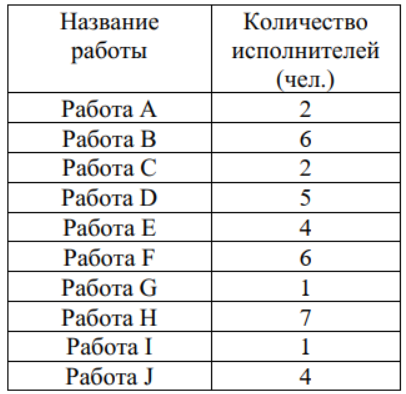
\includegraphics[width=0.7\linewidth]{task0_1}
	\caption{}
	\label{fig:task01}
\end{figure}

Призаданных условиях стоимость проекта составляет: 35805.71р, но силами 11 программистов сделать данный проект, при указанных условиях, невозможно (Смотрите изображение \ref{fig:task04}). Для выхода из данной ситуации есть несколько вариантов:
\begin{enumerate}
	\item Увеличить состав программистов (Не подходит по условиям задачи. Макс 11);
	\item Сдвинуть план с целью распределения \ref{fig:task03}.
\end{enumerate}

\begin{figure}[H]
	\centering
	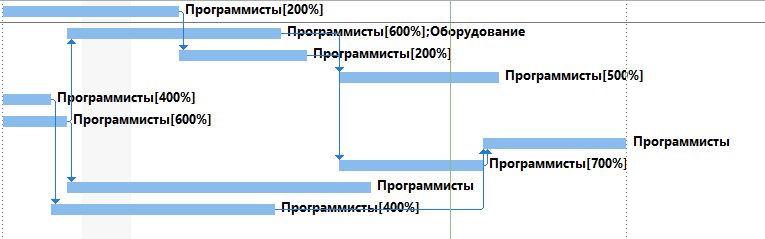
\includegraphics[width=0.7\linewidth]{src/task0_4}
	\caption{Изначальные сроки}
	\label{fig:task04}
\end{figure}
\begin{figure}[H]
	\centering
	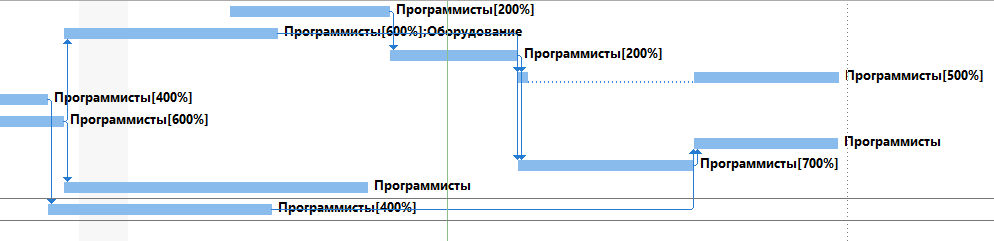
\includegraphics[width=0.7\linewidth]{src/task0_3}
	\caption{Обновленные}
	\label{fig:task03}
\end{figure}







